% Preamble - - - -
\documentclass[12pt]{article}
% Variables - - - -
\def\course{QSS 20}
\def\assignment{Short Essay}
\def\byline{}
\def\me{Roshan Karim}
\ifx\byline\empty
\def\subject{\course}
\else \def\subject{\course: \byline}
\fi
% - - - - Variables
% Commands - - - -
\newcommand{\opscale}[2]{\xrightarrow{#1r_#2 \text{→ } r_#2}}
\newcommand{\opreplace}[3]{\xrightarrow{r_#1 #2r_#3 \text{→ } r_#1}}
\newcommand{\opitc}[2]{\xrightarrow{r_#1 \text{↔} r_#2}}
% - - - - Commands
% Default Packages - - - -
\usepackage[letterpaper, total={6.5in, 9in}]{geometry}
\usepackage{fancyhdr}
\setlength{\headheight}{16pt}
\usepackage{titling}
\usepackage{citation-style-language}
\cslsetup{style = american-sociological-association}
\addbibresource{references.json}
\addbibresource{references.bib}
\usepackage[pdftitle={\assignment},
    pdfsubject={\subject},
    pdfauthor={\me},
    pdfproducer={LaTeX},
    pdfcreator={LuaLaTeX},
    colorlinks,
    citecolor=blue,
urlcolor=blue]{hyperref}
\usepackage{graphicx}
\graphicspath{{./images/}}
\usepackage{parskip}
\usepackage[all]{nowidow}
% - - - - Default Packages
% Unique Packages - - - -
\usepackage{amsmath}
\usepackage{txfonts}
\usepackage{fontspec}
\setmainfont{Charis SIL}
\usepackage{bm}
\usepackage{tikz}
\usepackage{pgfplots}
\pgfplotsset{compat=newest}
% - - - - Unique Packages
% Header - - - -
\pagestyle{fancy}
\lhead{\course: \assignment}
\chead{\me}
\rhead{\today}
% - - - - Header
% - - - - Preamble
\begin{document}
% Title - - - -
\begingroup
\centering
\ifx\byline\empty
\LARGE\assignment\\
\else\LARGE\assignment\\\large\byline\\[1.5em]
\fi
\endgroup
% - - - - Title
% Content - - - -
\section{Sociology and Transportation}
\subsection{What They Mean To Me}
I study Sociology and Mathematical Data Science, but I was born with a passion for transportation.
While the vehicles and the technology are fascinating, as I've explored the space, I've developed a familiarity and comfort with the complex systems that underlie transportation planning and urban development.
Since this past summer, beginning full-time and continuing part-time into the school year, I've been working at the Keolis Commuter Services, the operator of the MBTA Commuter Rail.
At this position, in my capacity as a Data Scientist, I've had the chance to explore much of the big data available to us as operators and consider how best to translate it for use by planners.
I consider myself an interpreter: while I lack fundamental domain knowledge, especially knowledge of railroad lingo, I have an important role to play in supporting those who do with data-driven insights.

\begin{figure}[h]
    \centering
    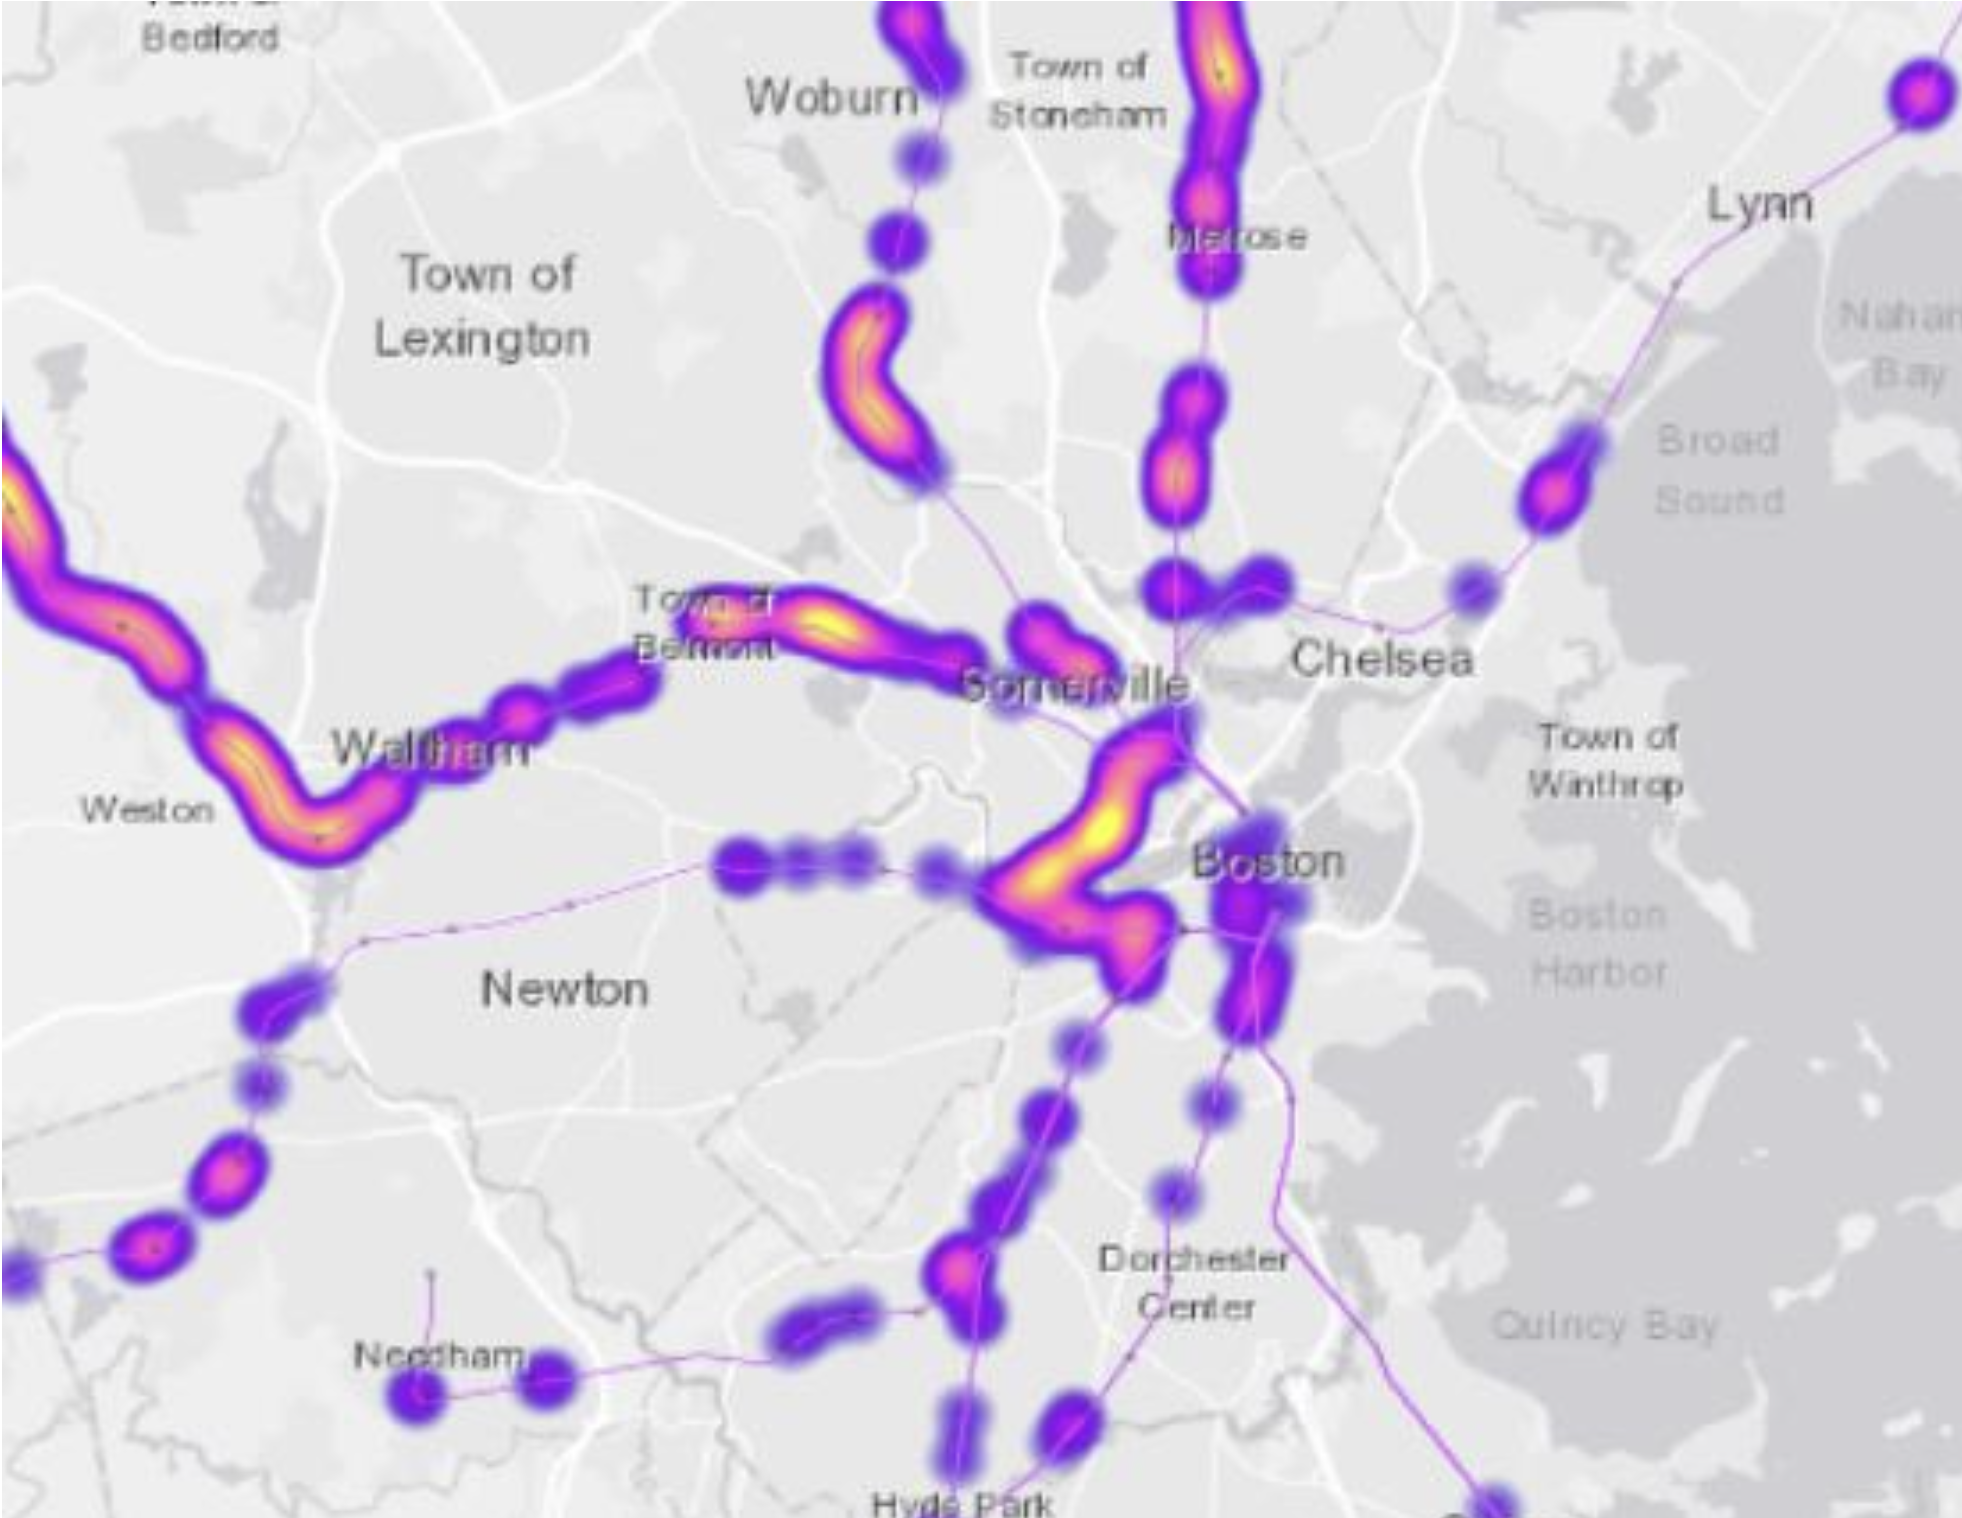
\includegraphics[width=0.5\textwidth]{images/heatmap.png}
    \caption{My first deliverable, a heatmap showing a bespoke 'slippery rail' metric I created using signals data from the last three years and machine learning techniques.}
\end{figure}

My general technique is to apply a research-driven approach to industry problems, which has made my work at Keolis somewhat novel.
Each project starts with a comprehensive literature review, which I often supplement with my own experimental data.
My slippery rail project started with a review of the process and contributing factors for low rail friction \cite{beagleyWheelRailAdhesion1975,chenWheelSlipSlide2020}.
I was privileged to be working with a large enough sample that true machine learning was not only possible, but optimal.
So, I took guidance from additional literature, such as \citet{steenisMonitoringTrainPerformance2010} on monitoring techniques, to craft an accurate model of network-level wheel slip to assist our Fall 2025 operations.

The takeaway here is that I find great interest in transportation networks more so than transit itself, and I hope to continue to apply sociological theory to understand the impacts our networks have on individuals and society.
\subsection{What I Want To Explore}
My work is primarily geospatial, so I expect my deliverable for this class to include some sort of map which accentuates a specific phenomenon (and of course, plenty of supporting figures).
Below, I will enumerate three sufficiently-narrow research topics, each with a specific research question I could endeavor to answer. 
\begin{enumerate}
    \item Transit Reliability and Spatial Inequality
        
        Reliable transportation determines if people can consistently reach work, school, healthcare, and other essential services.
        If service disruptions disproportionately affect disadvantaged communities, transportation systems can reinforce existing social and economic inequalities.
        Understanding these patterns can help transportation planners address system failures that have grave social consequence.
        In transportation, reliability is more important than frequency: a frequent, undependable service is of no use to the individuals who need it most.

    \textbf{Research Question:} Are Greater Boston MSA neighborhoods with higher socioeconomic disadvantage disproportionately affected by unreliable transit?

    Datasets include:
    \begin{itemize}
        \item ACS demographic data (from which multiple datasets must be used to build a Duncan Socioeconomic Index (SEI) for each tract) \\ \url{https://data.census.gov}.
        \item MBTA General Transit Feed Specification (GTFS) static data \\ \url{https://www.mbta.com/schedules-and-fares/developers/gtfs}.
        \item MBTA GTFS-realtime data available via my personal archive \\ \url{https://kcs-dataflows.karim.ac}.
    \end{itemize}    

    \item Employment and Transportation
    
        Access to reliable transportation shapes access to economic opportunity. 
        Even when jobs exist, long or difficult commutes can limit who can realistically reach them. 
        Measuring employment accessibility highlights geographic barriers to opportunity and helps policymakers identify where transit investments could improve social mobility and regional equity.
    
    \textbf{Research Question:} How does Greater Boston MSA transit accessibility shape access to employment opportunities in the MSA and the rest of Eastern Massachusetts? 

    Datasets include:
    \begin{itemize}
        \item Employment location data from the Longitudinal Employer-Household Dynamics (LEHD) program \\ \url{https://lehd.ces.census.gov}.
        \item MBTA General Transit Feed Specification (GTFS) static data \\ \url{https://www.mbta.com/schedules-and-fares/developers/gtfs}.
        \item MBTA GTFS-realtime data available via my personal archive \\ \url{https://kcs-dataflows.karim.ac}.
    \end{itemize}

    \item Weather, Infrastructure, and Socially-Determined Vulnerability
    
    Transportation disruptions caused by weather do not affect everyone equally. 
    Communities with fewer transportation alternatives often bear greater costs when rail service is unreliable. 
    Identifying where infrastructure failures intersect with social vulnerability can support more resilient transportation planning and reduce the unequal impacts of climate-related disruptions.

    \textbf{Research Question:} Do weather-related transit disruptions in the Greater Boston MSA disproportionately affect disadvantaged communities, socially vulnerable communities?

    Datasets include:
    \begin{itemize}
        \item Census Bureau data to construct a measure of vulnerability (could include Duncan SEI) \\ \url{https://data.census.gov}.
        \item MBTA General Transit Feed Specification (GTFS) static data \\ \url{https://www.mbta.com/schedules-and-fares/developers/gtfs}.
        \item MBTA GTFS-realtime data available via my personal archive \\ \url{https://kcs-dataflows.karim.ac}.
        \item ERA5 Reanalysis data from the European Centre for Medium-Range Weather Forecasts (ECMWF) \\ \url{https://cds.climate.copernicus.eu/datasets/reanalysis-era5-single-levels}.
    \end{itemize}
\end{enumerate}
\subsection{What I'll Bring}
I like transportation. I like thinking about it, analyzing it, using it, and improving it.
The path I'll take through this world remains to-be-determined, as it will for a while.
I know I'll explore industry (through my work at Keolis and others), but I'm seriously contemplating an eventual transition to academia.
So, right now, the only thing that I can commit to bringing to this world is a few more data-driven insights that, left in the right hands, can improve my community in Greater Boston and our national understanding of the importance of transportation.
I am a far cry away from achieving this independently, but I am already aware of the positive impacts my work has had for the Commuter Rail as the result of the support of the Keolis Executive Team.
One day, I may be significant enough to have impact as an individual, but today, it is just about seeking to exist in the right place at the right time with the right people to drive change.
\section{On Generative AI}
I can confidently state that I do not know enough to evaluate the net impact of generative AI on society.
I am certain of this fact because I believe that quantity to be currently unmeasurable.
Whatever impact it has, it is here to stay, and the study of its medium to long-term effects is left to myself in my senior years or, more fruitfully, to the next generation of scholars.

That said, I am confident that generative AI is a net positive in my life.
I am fundamentally a member of the core group which stands to benefit the most from generative AI.
I am intelligent and successful enough to be shielded from the career risks of generative AI, and with my knowledge of AI/ML, I can meaningfully contribute to the field.
Knowing all of this, there is a question to be answered about the impact of AI on social inequality.
I will draw out an example from my studies in the sociology of health.
On a consistent basis, technological advances in medicine improve overall health outcomes, but they always do so more for the advantaged than the disadvantaged.
Technology exacerbates inequality through access and adoption, and the more significant the technology, the greater the response.
If AI is to be the most significant technological advance in human history, we have an opportunity to exacerbate inequalities to a novel degree, for which the consequences remain uncertain.
\subsection{My AI Use}
I use generative AI religiously for work, and almost all my code is written, checked by, or workshopped using a large language model.
The release of Claude Code was when I finally cracked and began heavy use of generative AI in programming, though I am currently using OpenAI Codex.
I use AI so much for work because the tasks that I perform are no longer fundamental knowledge that I believe is necessary to learn, but specific implementation minutia that I am unlikely to make use of again in the same way.
Essentially, I learn tools and theory, not implementations.

Logically, I am scared of using generative AI for school. 
I believe much of the work of an undergraduate education is to learn the theory, not the practice, and to build intuition and understanding.
If I make heavy use of models, I fear that I am setting myself up for failure in the future.
In a well-taught Dartmouth course, nothing should be so specific as to be assumed useless to my future.
And I am not an educator, so I am left to place my trust in the pedagogy of my instructor.
Thus, I exclusively adhere to my course's generative AI guidelines, not just because those are the rules, but because I believe my knowledge is more limited than that of my instructor.

Some common uses of generative AI in my school work include initial research and literature review and proofreading/revision.
I find that I produce a higher quality written output when I build a framework for GPT to support through revision, rather than starting with a model's output.
In these processes, I feel empowered to retain ownership of my work and learning while also making use of this technology to improve my understanding and the quality of my work.
\section{The World Cup}
When games are played in Boston, I support whichever team has fewer fans\dots coordinating the transportation of 20,000 fans to and from the stadium, which is the minimum number my company has transported to a game, is definitely a stress test, and even as a low-level employee I contribute to ad-hoc service optimization on game days.
But otherwise, I support the U.S. Men's National Team.
Though our country has its flaws, and it is sometimes hard to remain optimistic about our future, I am an American, born and raised, and I believe that I have a responsibility to retain hope for the country I call my home.
\printbibliography
I generated these citations using the citation-style-language package and a heavily corrected version of the American Sociological Association CSL created by the maintainers of Zotero.
I find that this is the best way to ensure deterministic generation of citations that (with a well-crafted CSL) are guaranteed to be consistent with style guidelines for the source types I implement.
Please do advise me if there is a better way to accomplish strict consistency with style guidelines, as this process is kind of inconvenient when adopting a new style.
% - - - - Content
\end{document}